\documentclass[a4paper,12pt]{article}
\usepackage[french]{babel}
\usepackage[utf8]{inputenc}
\usepackage[T1]{fontenc}
\usepackage{graphicx}
\usepackage{hyperref}
\usepackage{svg}
\usepackage{titlesec}
\usepackage{geometry}
\usepackage{enumitem}
\usepackage{tikz}
\usetikzlibrary{shapes,arrows}

\titlespacing*{\section}{0pt}{*0.5}{*0.25}
\titlespacing*{\subsection}{0pt}{*0.25}{*0.125}
\setlist[itemize]{itemsep=0pt, topsep=0pt}

% Define a new level of subsection
\titleclass{\subsubsubsection}{straight}[\subsubsection]
\newcounter{subsubsubsection}[subsubsection]
\renewcommand\thesubsubsubsection{\thesubsubsection.\arabic{subsubsubsection}}
\titleformat{\subsubsubsection}
  {\normalfont\normalsize\bfseries}{\thesubsubsubsection}{1em}{}
\titlespacing*{\subsubsubsection}
  {0pt}{1.25ex plus 1ex minus .2ex}{0.5ex plus .2ex}

\title{Rapport du Projet \\ \textbf{FindMyTech}}
\author{Mouadh Belgoumri (Team Leader, Frontend) \\ Abdelouadoude Sahnoune (Frontend) \\ Khaled Houari (Backend) \\ Arab Mehdi (Backend) \\ Cheurfa Aimed (UI/UX) \\ Zinnedine Zitouni (UI/UX) \\ Encadré par : Mdm. Feriel Khennouche}
\date{\today}

\begin{document}

\maketitle
\tableofcontents

\section{Titre du projet}
FindMyTech

\section{Contexte et justification}
L'achat d'équipements informatiques peut être complexe en raison de la diversité des produits et des spécifications techniques. FindMyTech vise à simplifier ce processus en fournissant un comparateur de produits performant avec une boutique intégrée permettant l'achat direct.

\section{Objectifs du projet}
\begin{itemize}
    \item Développer une plateforme intuitive permettant aux utilisateurs de comparer facilement des équipements informatiques.
    \item Offrir une base de données centralisée regroupant des fiches techniques détaillées.
    \item Permettre un filtrage avancé selon les catégories et budgets.
    \item Intégrer un magasin en ligne facilitant l'achat direct des produits comparés.
\end{itemize}

\section{Acteurs du système}
\subsection{Administrateur}
\begin{itemize}
    \item Gestion des produits et des catégories.
    \item Supervision des commandes et des transactions.
    \item Maintenance de la plateforme et gestion des utilisateurs.
\end{itemize}

\subsection{Acheteur}
\begin{itemize}
    \item Recherche et comparaison de produits.
    \item Ajout de produits favoris et suivi des prix.
    \item Achat direct via le magasin intégré.
\end{itemize}

\subsection{Vendeur}
\begin{itemize}
    \item Gestion du stock et des prix.
    \item Réception et gestion des commandes clients.
    \item Interaction avec l’administration pour la mise en ligne des produits.
\end{itemize}

\section{Technologies utilisées}
\begin{itemize}
    \item \textbf{Frontend} : HTML, CSS, JavaScript.
    \item \textbf{Backend} : Php, Laravel.
    \item \textbf{Base de données} : SQL.
    \item \textbf{UI/UX} : Figma.
    \item \textbf{API externes} : récupération des informations techniques des produits.
\end{itemize}

\section{Architecture du projet}
FindMyTech suit une architecture MVC (Modèle-Vue-Contrôleur) garantissant une séparation claire entre la logique métier, l'affichage et la gestion des données.

\section{Contraintes et exigences}
\subsection{Contraintes Techniques}
\begin{itemize}
    \item Compatibilité avec les navigateurs modernes.
    \item Temps de réponse optimisé.
    \item Interface utilisateur fluide et réactive.
\end{itemize}

\subsection{Contraintes de Sécurité}
\begin{itemize}
    \item Sécurisation des paiements et des transactions.
    \item Protection des données des utilisateurs.
    \item Authentification sécurisée avec JWT.
\end{itemize}

\subsection{Contraintes Ergonomiques}
\begin{itemize}
    \item Interface intuitive et accessible pour tous les utilisateurs.
    \item Navigation fluide et structurée.
\end{itemize}

\section{Phases du projet}
\begin{itemize}
    \item \textbf{Phase 1} : Analyse et conception (schéma de base de données, maquettes UI/UX).
    \item \textbf{Phase 2} : Développement des fonctionnalités principales.
    \item \textbf{Phase 3} : Tests et corrections des bugs.
    \item \textbf{Phase 4} : Présentation finale et soumission du rapport.
\end{itemize}

\section{Livrables attendus}
\begin{itemize}
    \item Code source documenté.
    \item Rapport technique du projet.
    \item Présentation orale et démonstration de la plateforme.
\end{itemize}

\section{Diagrammes UML}
\subsection{Diagramme de cas d'utilisation}
\subsubsection{Cas d'utilisation principaux}

\subsection{Pour l'Acheteur}
\begin{itemize}
    \item \textbf{Créer un compte} : L'utilisateur peut s'inscrire sur la plateforme.
    \item \textbf{Se connecter} : Il doit s'authentifier avant d'accéder à certaines fonctionnalités.
    \item \textbf{Changement des données personnelles} : Il peut modifier ses informations personnelles après connexion.
    \item \textbf{Recherche et filtrage} : Il peut rechercher un produit en utilisant des filtres spécifiques.
    \item \textbf{Comparaison} : Il peut comparer plusieurs produits en fonction de leurs caractéristiques.
    \item \textbf{Paiement} : Après avoir sélectionné un produit, il peut procéder au paiement.
    \begin{itemize}
        \item \textit{\textbf{<<include>> Vérifier la suffisance des fonds}} : Avant la validation du paiement, le système vérifie que l'utilisateur dispose des fonds nécessaires.
        \subsubsubsection{Détails de la vérification des fonds}
        \begin{itemize}
            \item Vérification du solde disponible.
            \item Vérification des limites de transaction.
        \end{itemize}
    \end{itemize}
    \item \textbf{Afficher une erreur d'authentification} : Si l'identification échoue, un message d'erreur s'affiche.
\end{itemize}

\subsection{Pour le Vendeur}
\begin{itemize}
    \item \textbf{Mettre un nouveau produit} : Le vendeur peut ajouter un produit à vendre sur la plateforme.
    \item \textbf{Retirer son produit} : Il peut supprimer ses propres produits.
    \item \textbf{Consulter l'état du stock} : Il peut vérifier l’état du stock des produits qu’il vend.
\end{itemize}

\subsection{Pour l'Admin}
\begin{itemize}
    \item \textbf{Consulter les statistiques} : L'admin a accès aux statistiques globales de la plateforme.
    \item \textbf{Consulter la liste des vendeurs} : Il peut voir les vendeurs enregistrés.
    \item \textbf{Modifier les produits (suppression et ajout)} : Il peut gérer les produits disponibles sur la plateforme.
\end{itemize}

\section{Relations entre les cas d'utilisation}
\begin{itemize}
    \item \textbf{<<include>> Vérifier la suffisance des fonds} est inclus dans le cas d'utilisation \textbf{Paiement}, car il s'agit d'une étape obligatoire pour valider une transaction.
    \item \textbf{<<extend>> Afficher une erreur d'authentification} est une extension du cas \textbf{Se connecter}, activée uniquement en cas d’échec de l’authentification.
\end{itemize}

\begin{figure}
    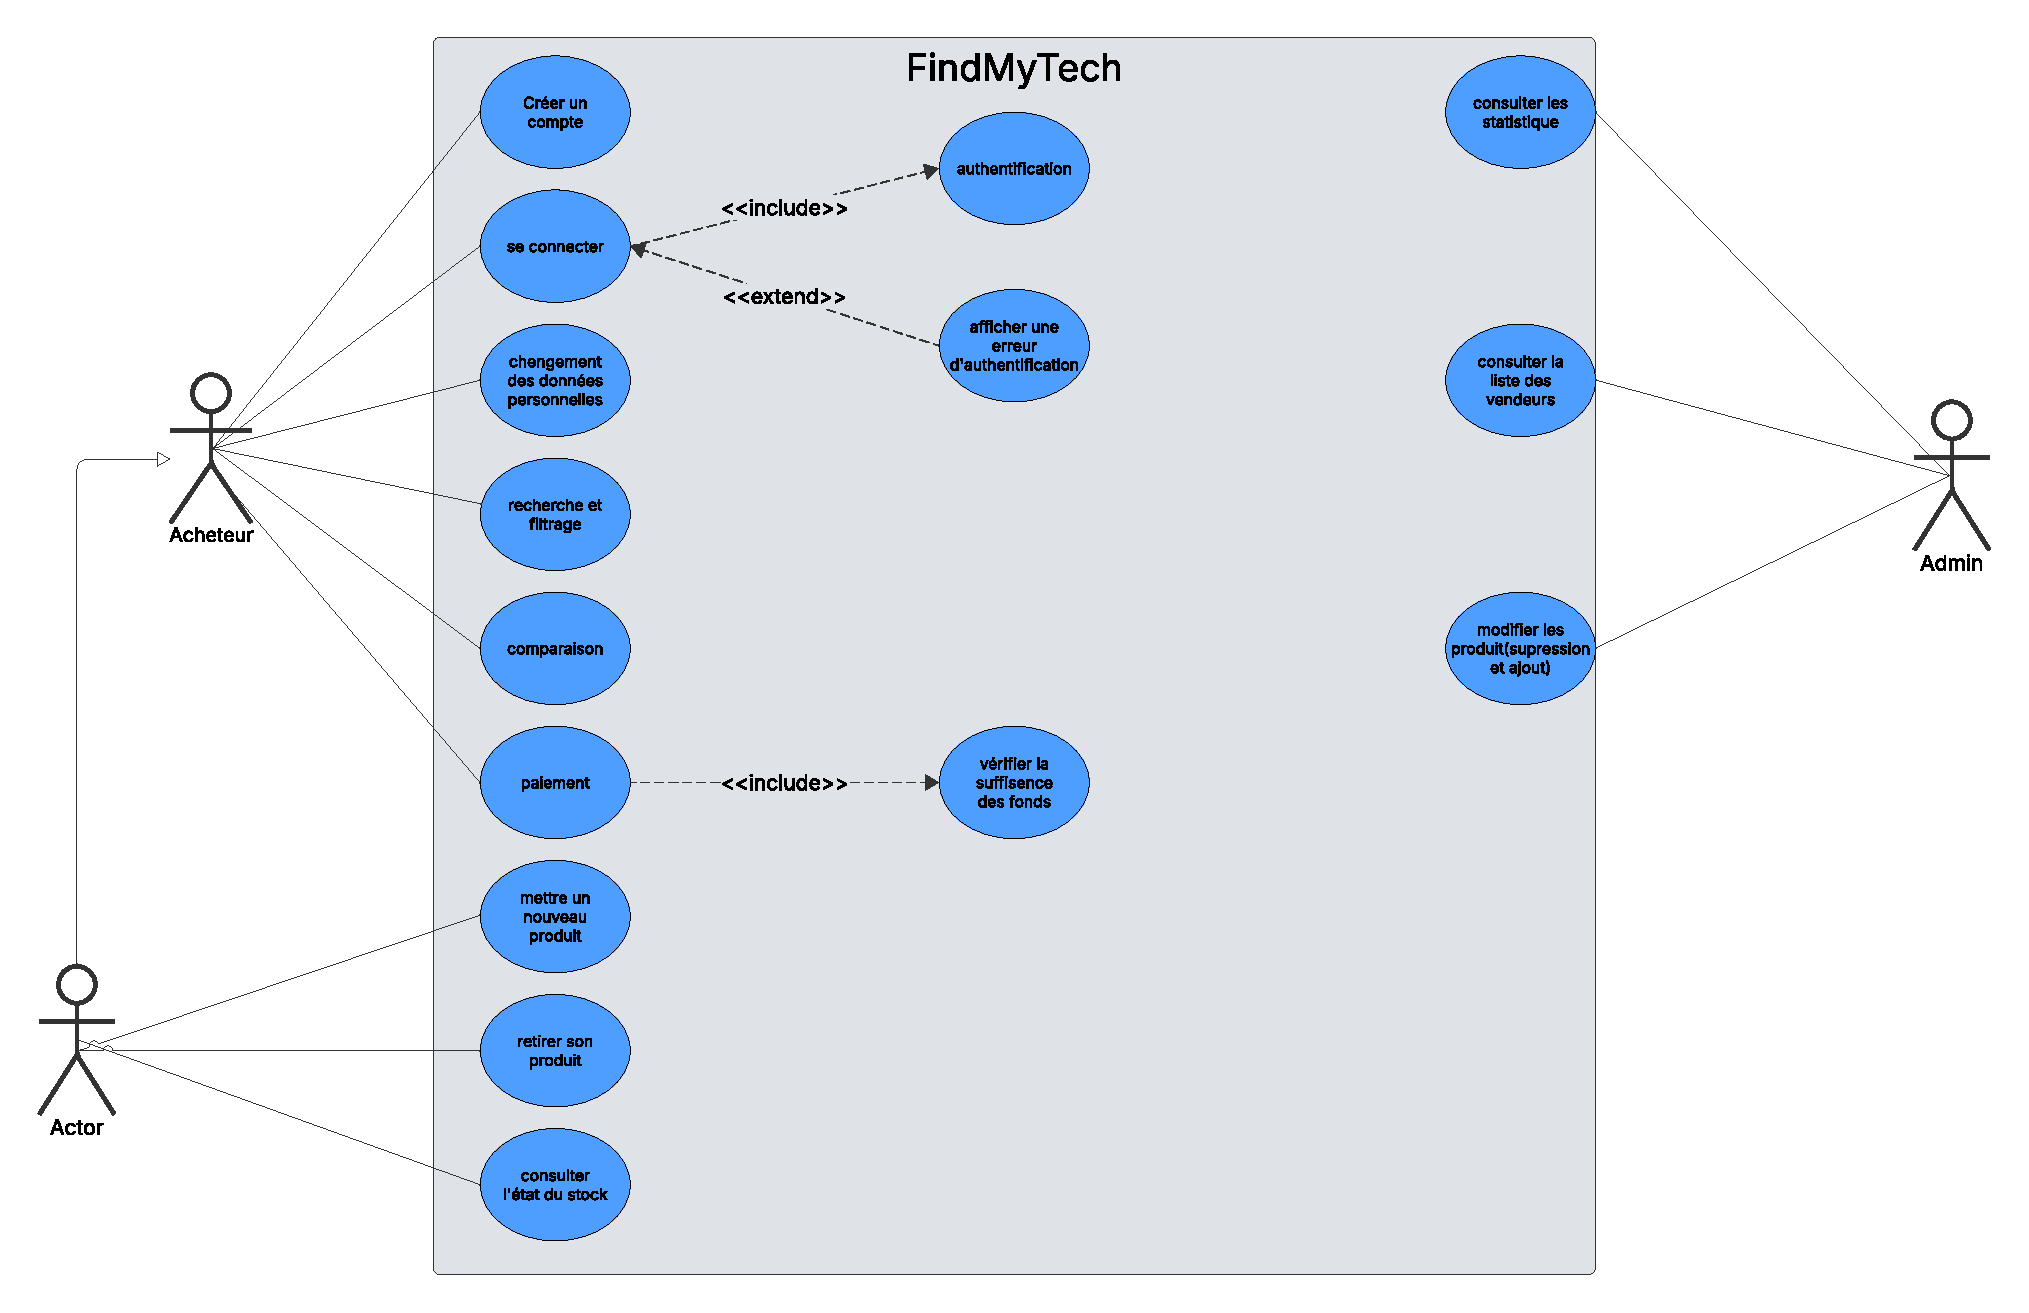
\includegraphics[width=\textwidth]{out/diagrammes/diagramme_des_cas d'utilisation.pdf}
    \caption{Diagramme de cas d'utilisation}
\end{figure}

\clearpage

\subsection{Diagramme de séquence}
Ce diagramme illustre les interactions dynamiques entre les utilisateurs, le système et la base de données, mettant en évidence le processus de comparaison et d’achat.
\begin{figure}
    \centering
    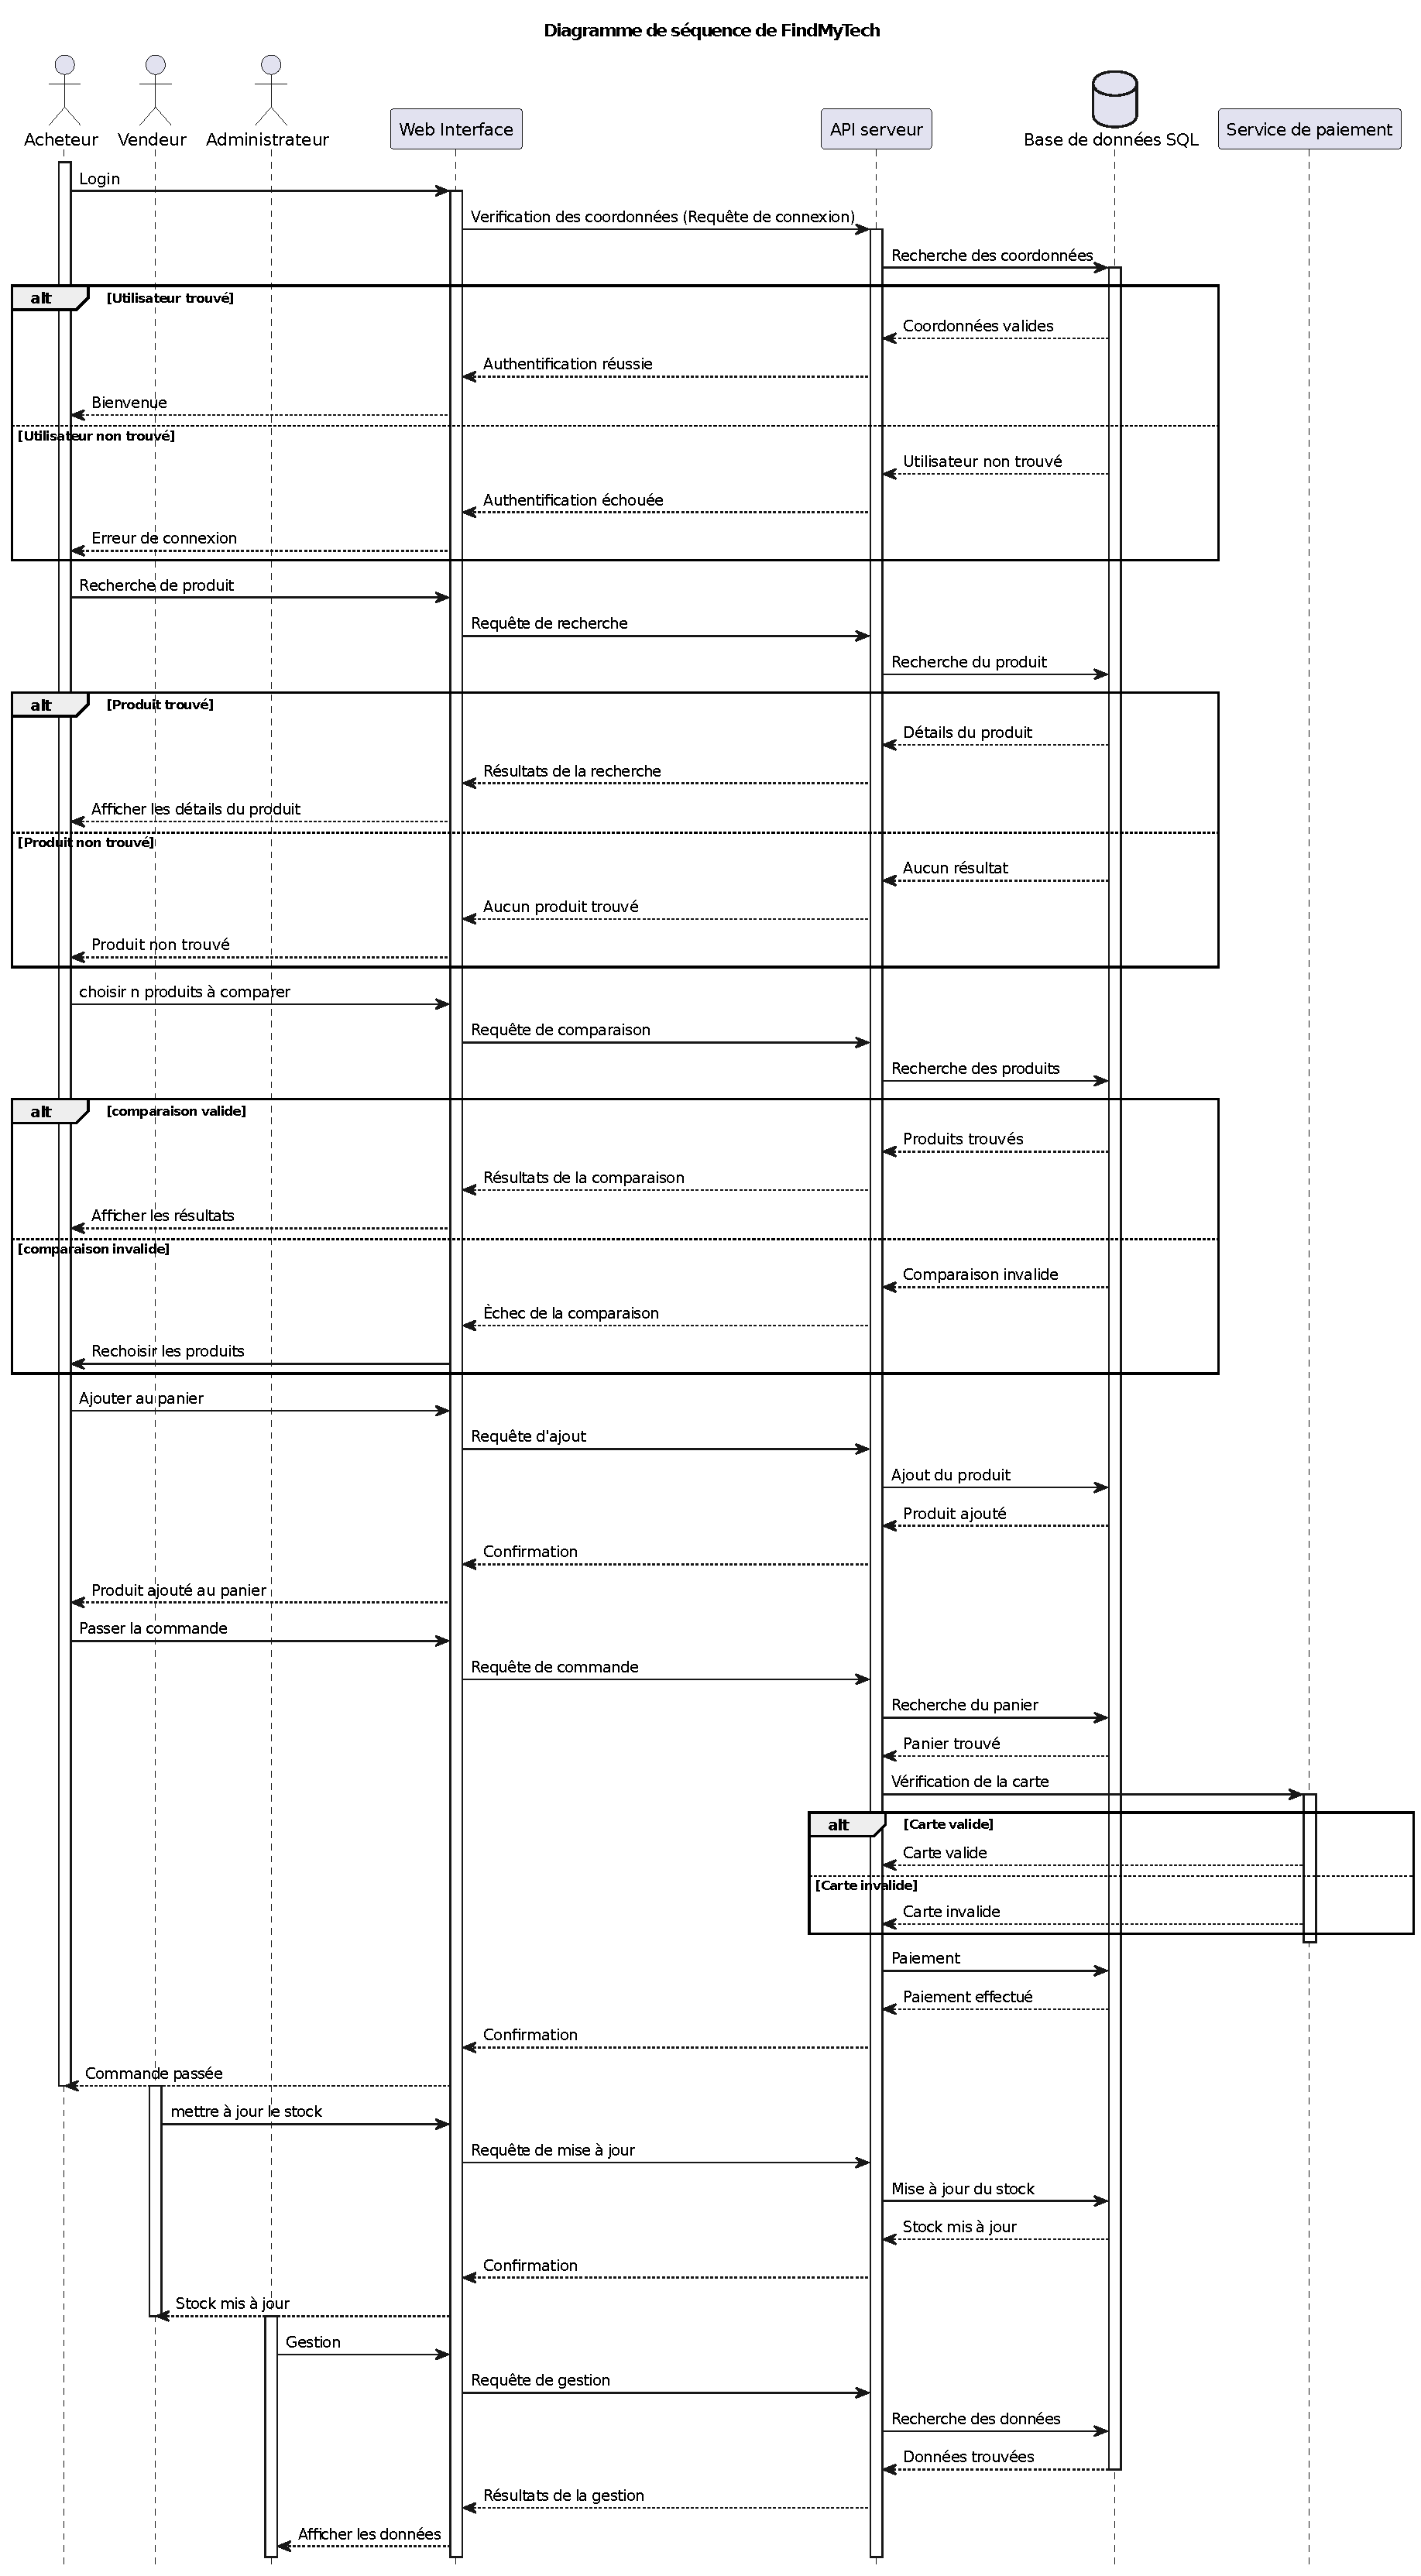
\includegraphics[width=0.8\textwidth]{out/diagrammes/diagramme_de_sequence.pdf}
    \caption{Diagramme de séquence}
\end{figure}

\clearpage

\subsection{Diagramme de classes}
Il détaille la structure du projet en mettant en évidence les classes principales et leurs relations, incluant les classes \textit{Produit}, \textit{Utilisateur}, \textit{Commande}, et \textit{Panier}.

\section{Description des classes}
\subsection{Classe Utilisateur}
\textbf{Attributs} :
\begin{itemize}
    \item \texttt{UserId} : int – Identifiant unique de l'utilisateur.
    \item \texttt{Password} : string – Mot de passe pour l'authentification.
\end{itemize}
\textbf{Méthodes} :
\begin{itemize}
    \item \texttt{Créer un compte()} – Permet de créer un compte utilisateur.
    \item \texttt{se connecter()} – Authentifie l'utilisateur.
    \item \texttt{mettre\_à\_jour\_le\_profil()} – Met à jour les informations personnelles.
\end{itemize}

\subsection{Classe Acheteur (Hérite de Utilisateur)}
\textbf{Attributs} :
\begin{itemize}
    \item \texttt{Nom} : string – Nom de l'acheteur.
    \item \texttt{Prénom} : string – Prénom de l'acheteur.
    \item \texttt{Adresse} : string – Adresse de livraison.
\end{itemize}
\textbf{Méthodes} :
\begin{itemize}
    \item \texttt{ajouter\_au\_panier()} – Ajoute un produit au panier.
    \item \texttt{passer\_une\_commande()} – Finalise une commande.
\end{itemize}

\subsection{Classe Vendeur (Hérite de Utilisateur)}
\textbf{Attributs} :
\begin{itemize}
    \item \texttt{adresse\_de\_magasin} : string – Adresse du magasin du vendeur.
\end{itemize}
\textbf{Méthodes} :
\begin{itemize}
    \item \texttt{mettre\_à\_jour\_son\_stock()} – Permet de modifier les stocks disponibles.
\end{itemize}

\subsection{Classe Administrateur (Hérite de Utilisateur)}
\textbf{Attributs} :
\begin{itemize}
    \item \texttt{SuperID} : int – Identifiant spécifique de l'administrateur.
\end{itemize}
\textbf{Méthodes} :
\begin{itemize}
    \item \texttt{gestion\_de\_BD()} – Gestion de la base de données.
    \item \texttt{consulter\_liste\_vendeurs()} – Affiche la liste des vendeurs enregistrés.
    \item \texttt{consulter\_ventes()} – Affiche les ventes réalisées.
\end{itemize}

\subsection{Classe Panier}
\textbf{Attributs} :
\begin{itemize}
    \item \texttt{listeDesIdProduits[]} : int – Liste des identifiants des produits ajoutés.
    \item \texttt{prixUnit} : int – Prix unitaire d'un produit.
    \item \texttt{total} : int – Prix total du panier.
\end{itemize}
\textbf{Méthodes} :
\begin{itemize}
    \item \texttt{ajouter\_au\_panier()} – Ajoute un produit au panier.
    \item \texttt{consulterPanier()} – Affiche le contenu du panier.
\end{itemize}

\subsection{Classe Commande}
\textbf{Attributs} :
\begin{itemize}
    \item \texttt{IdCommande} : int – Identifiant unique de la commande.
    \item \texttt{NomClient} : string – Nom du client ayant passé la commande.
    \item \texttt{dateDeCommande} : string – Date de la commande.
\end{itemize}
\textbf{Méthodes} :
\begin{itemize}
    \item \texttt{passer\_une\_commande()} – Permet de finaliser une commande.
\end{itemize}

\subsection{Classe CarteDePaiement}
\textbf{Attributs} :
\begin{itemize}
    \item \texttt{NuméroDuCarte} : int – Numéro unique de la carte bancaire.
    \item \texttt{codePinDeCarte} : int – Code PIN de la carte.
    \item \texttt{montantActuel} : int – Solde disponible sur la carte.
\end{itemize}
\textbf{Méthodes} :
\begin{itemize}
    \item \texttt{paiement()} – Effectue un paiement à partir de la carte.
\end{itemize}
\begin{figure}
    \centering
    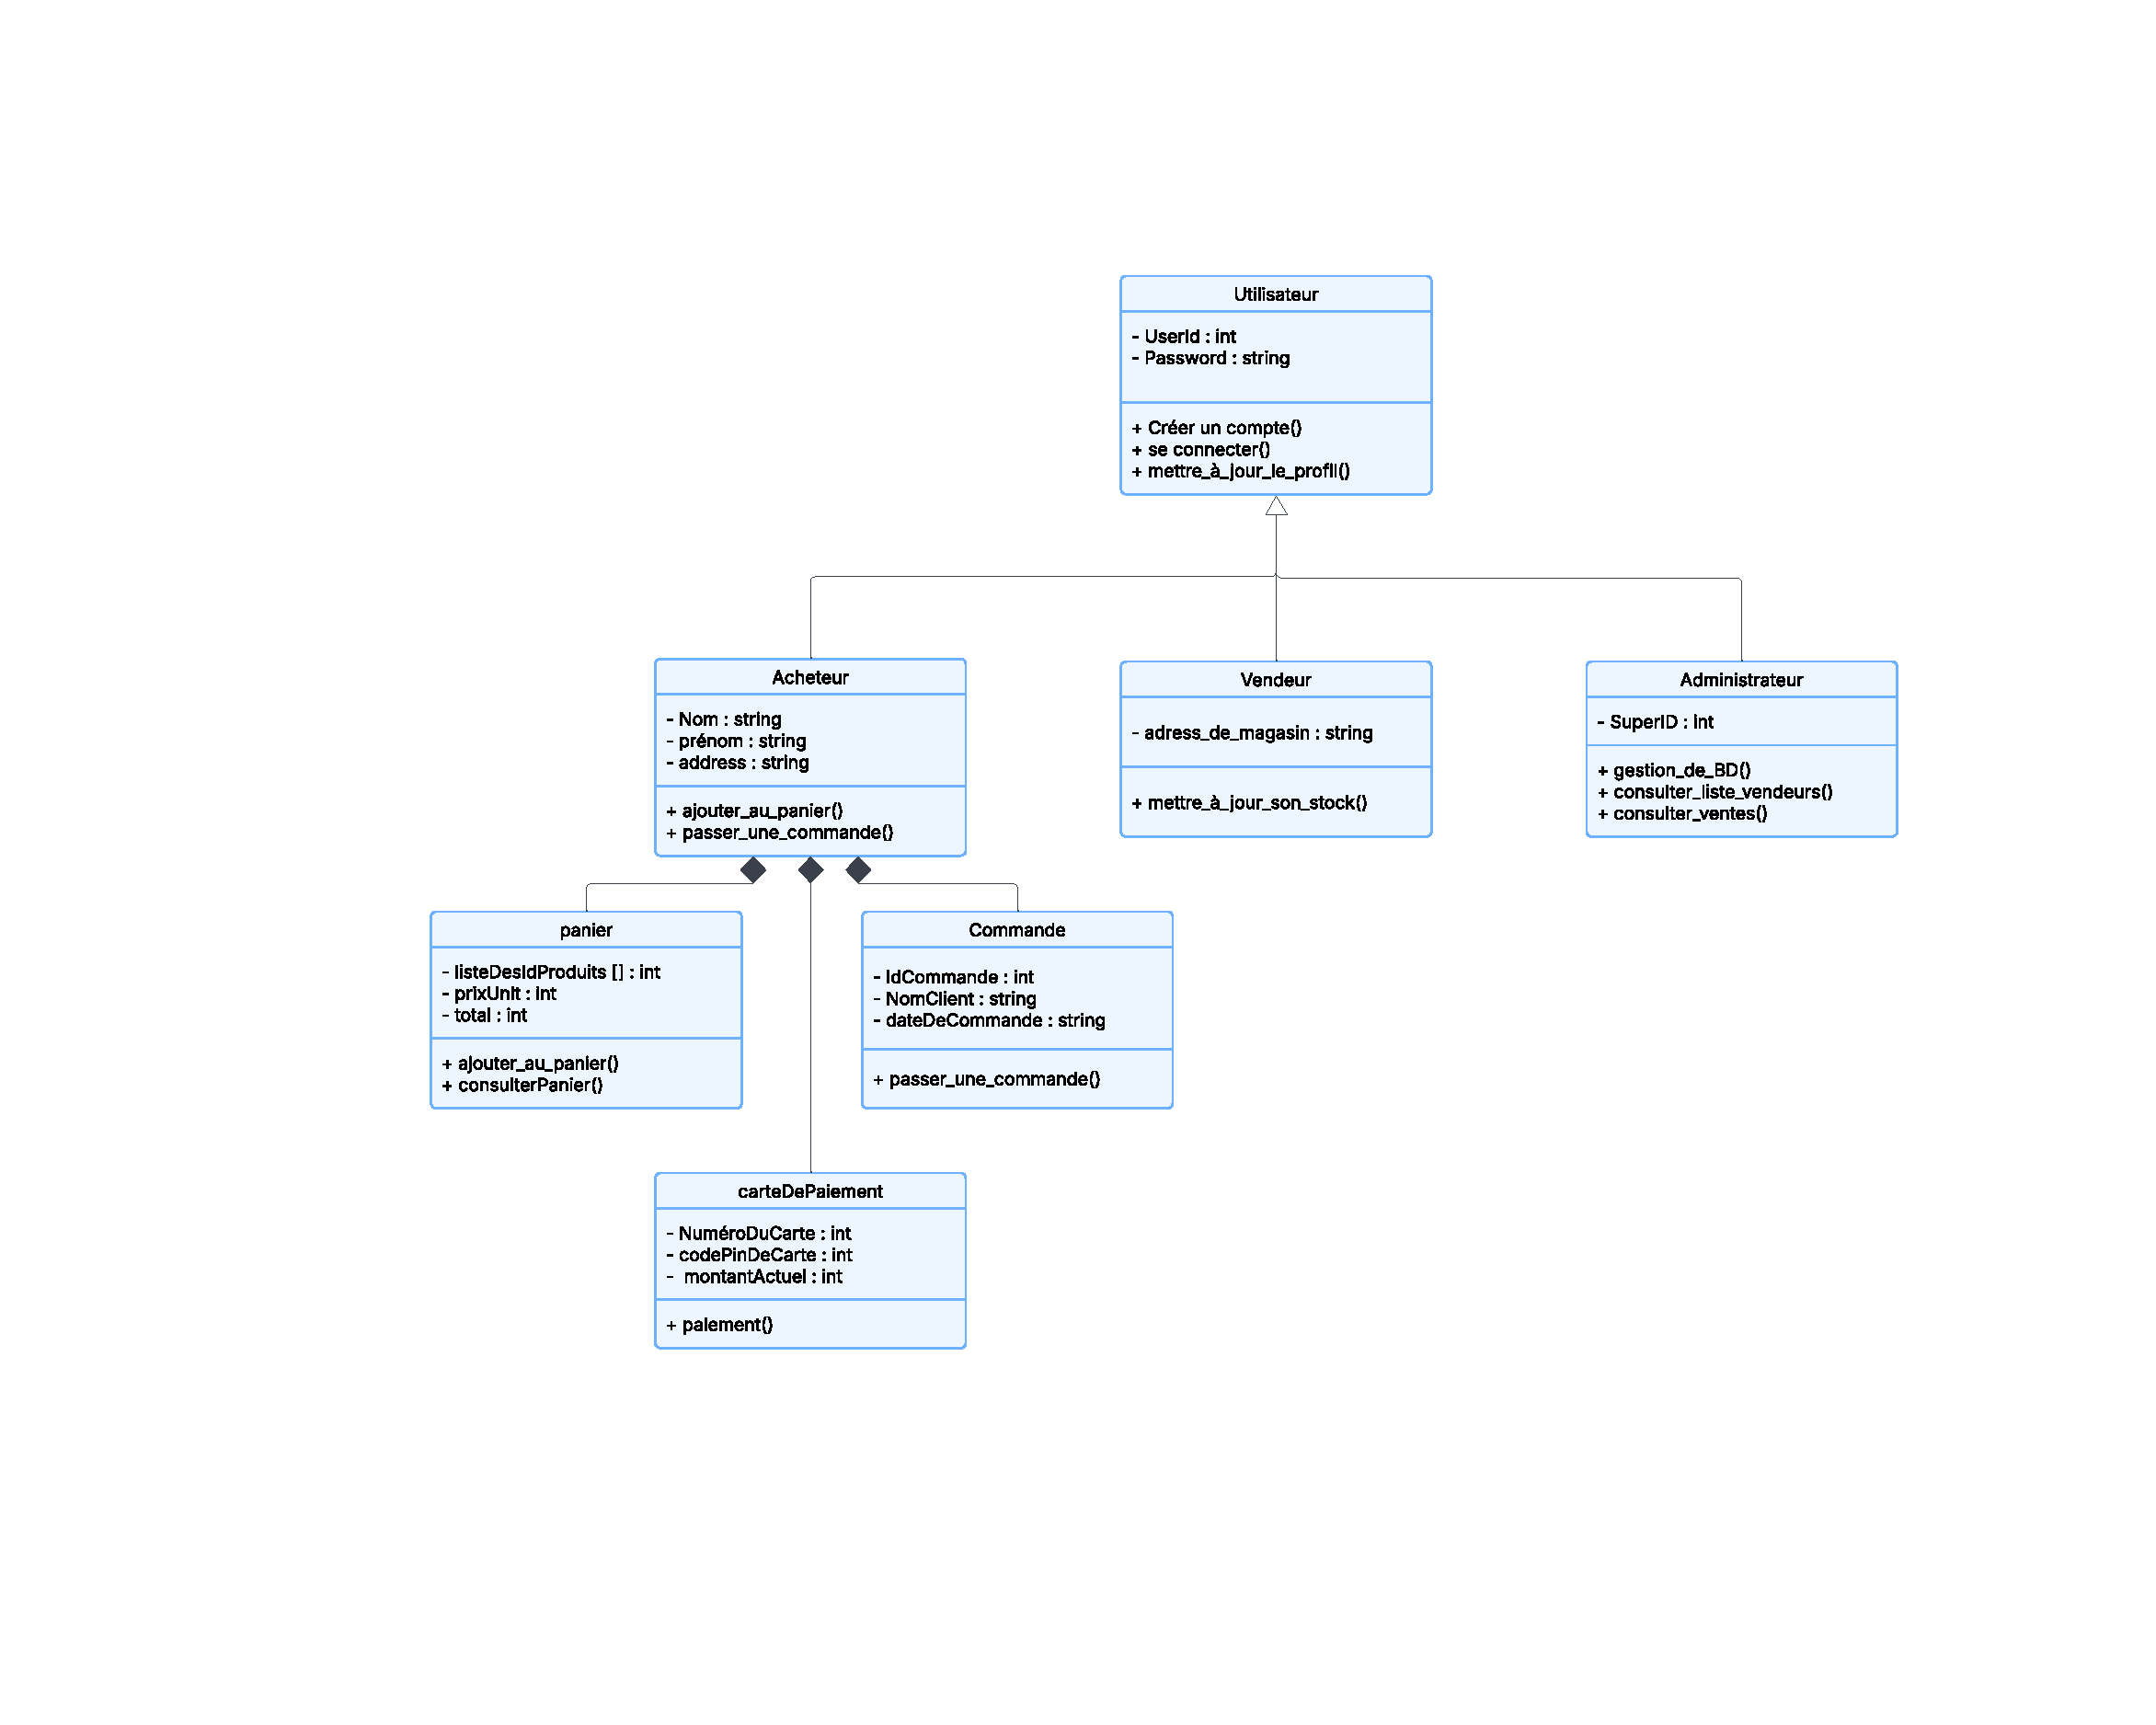
\includegraphics[width=0.8\textwidth]{out/diagrammes/Diagramme_des_classes.pdf}
    \caption{Diagramme de classes}
\end{figure}

\clearpage

\subsection{Diagramme d’architecture}
Ce diagramme présente la structure logicielle du projet, mettant en avant la séparation entre l’interface utilisateur, la logique métier et la gestion des données.
\begin{figure}
    \centering
    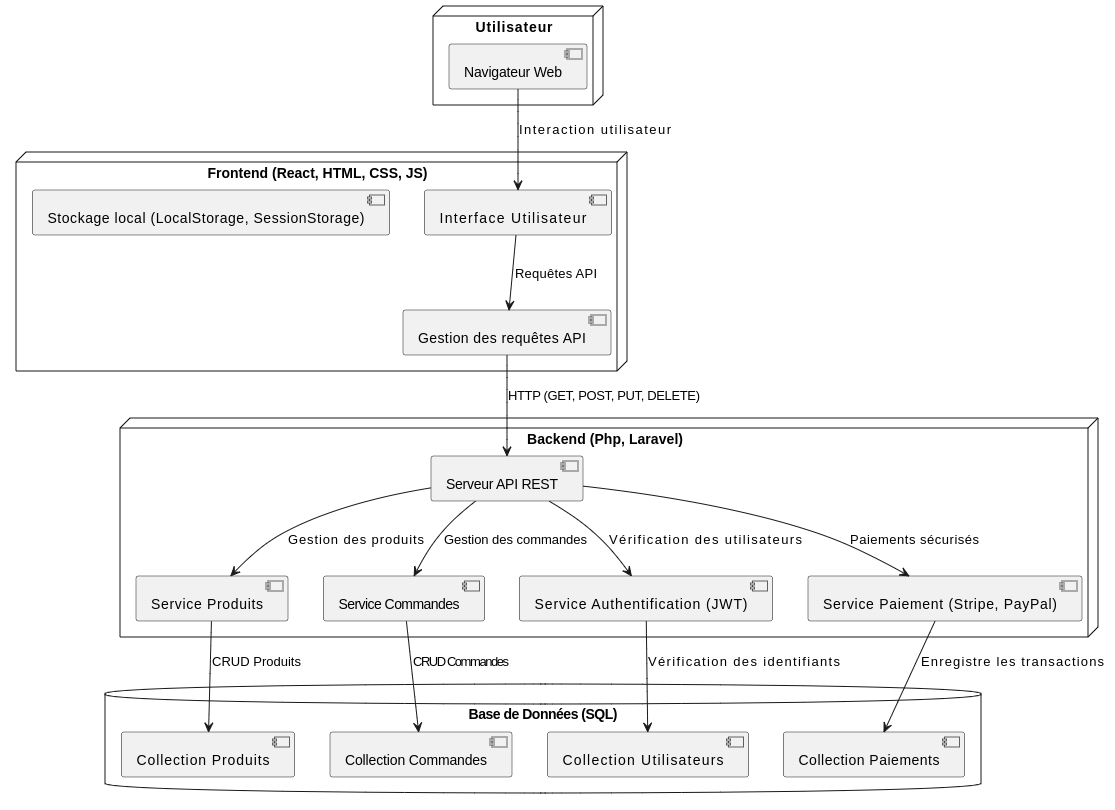
\includegraphics[width=\textwidth]{out/diagrammes/archi3.png}
    \caption{Diagramme d'architecture}
\end{figure}

\section{Composants principaux}
Le système est divisé en trois parties principales :
\begin{itemize}
    \item \textbf{Frontend} (React, HTML, CSS, JS) : Interface utilisateur qui permet l’interaction avec le système.
    \item \textbf{Backend} (PHP, Laravel) : Serveur qui traite les requêtes et gère la logique métier.
    \item \textbf{Base de données} (SQL) : Stocke les informations essentielles comme les produits, commandes, utilisateurs et paiements.
\end{itemize}

\section{Description détaillée}
\subsection{Utilisateur}
L'utilisateur interagit avec le système via un \textbf{navigateur web}. Toutes les actions passent par l'interface utilisateur du frontend.

\subsection{Frontend}
Le frontend est développé avec \textbf{React, HTML, CSS et JavaScript}. Il contient plusieurs composants :
\begin{itemize}
    \item \textbf{Interface utilisateur} : Affiche les pages web et gère l’interaction avec l’utilisateur.
    \item \textbf{Stockage local (LocalStorage, SessionStorage)} : Permet de stocker temporairement certaines données utilisateur.
    \item \textbf{Gestion des requêtes API} : Envoie des requêtes au backend via HTTP (\texttt{GET, POST, PUT, DELETE}).
\end{itemize}

\subsection{Backend}
Le backend est développé en \textbf{PHP (Laravel)} et est responsable de la gestion des données et des requêtes. Il est composé de :
\begin{itemize}
    \item \textbf{Serveur API REST} : Point central de communication entre le frontend et la base de données.
    \item \textbf{Service Produits} : Gère les produits et leurs caractéristiques (CRUD Produits).
    \item \textbf{Service Commandes} : Gère les commandes des utilisateurs (CRUD Commandes).
    \item \textbf{Service Authentification (JWT)} : Vérifie les utilisateurs et gère la connexion sécurisée.
    \item \textbf{Service Paiement (Stripe, PayPal)} : Assure la gestion des transactions financières sécurisées.
\end{itemize}

\subsection{Base de Données (SQL)}
La base de données stocke toutes les informations nécessaires :
\begin{itemize}
    \item \textbf{Collection Produits} : Stocke les informations sur les produits disponibles.
    \item \textbf{Collection Commandes} : Contient les détails des commandes effectuées.
    \item \textbf{Collection Utilisateurs} : Enregistre les comptes utilisateurs et leurs informations.
    \item \textbf{Collection Paiements} : Archive les transactions et paiements réalisés.
\end{itemize}

\section{Conclusion}
Cette architecture garantit une séparation claire entre les différentes couches du système et assure une communication fluide entre le frontend, le backend et la base de données. Grâce à cette structuration, \textbf{FindMyTech} peut offrir une expérience utilisateur fluide, sécurisée et efficace.
\section{Justification Des Technologies utilisées}
\subsection{Frontend}
Le frontend est la partie visible du site web avec laquelle l’utilisateur interagit. Pour garantir une interface fluide, moderne et réactive, nous avons opté pour les technologies suivantes :

\begin{itemize}
    \item \textbf{React.js} : Bibliothèque JavaScript pour la construction d’interfaces utilisateur.
    \item \textbf{Bootstrap} : Framework CSS permettant de créer des designs responsifs rapidement.
    \item \textbf{Sass} : Préprocesseur CSS facilitant l’écriture et la gestion des styles.
\end{itemize}

\subsection{Backend}
Pour la gestion des requêtes et des données, nous avons choisi :

\begin{itemize}
    \item \textbf{PHP} : Langage de programmation utilisé pour le développement backend.
    \item \textbf{Laravel} : Framework PHP facilitant le développement d’applications web robustes et sécurisées.
    \item \textbf{SQL} : Système de gestion de bases de données relationnelles.
\end{itemize}

\section{Justification des choix technologiques}
\subsection{Pourquoi React.js ?}
\textbf{React.js} est une bibliothèque JavaScript développée par Facebook et largement utilisée pour créer des interfaces utilisateur dynamiques et performantes.

\textbf{Avantages :}
\begin{itemize}
    \item \textbf{Composants réutilisables} : Permet de structurer l’interface en éléments indépendants et réutilisables.
    \item \textbf{Performance optimisée} : Grâce au \textit{Virtual DOM}, React réduit le nombre de mises à jour réelles du DOM, améliorant ainsi la fluidité de l’application.
    \item \textbf{Grande communauté et support} : Un écosystème riche avec de nombreuses bibliothèques et ressources disponibles.
    \item \textbf{Facilité d’intégration} : Compatible avec d’autres technologies comme \textit{Redux}, \textit{React Router} et \textit{Axios}.
\end{itemize}

\subsection{Pourquoi Bootstrap ?}
\textbf{Bootstrap} est un framework CSS populaire qui permet de créer rapidement des interfaces responsives et attrayantes.

\textbf{Avantages :}
\begin{itemize}
    \item \textbf{Développement rapide} : Contient des composants prêts à l’emploi (boutons, formulaires, alertes, etc.).
    \item \textbf{Responsive par défaut} : Utilise une grille flexible qui s’adapte aux différents écrans.
    \item \textbf{Compatibilité élevée} : Fonctionne sur tous les navigateurs modernes sans nécessiter d’adaptations complexes.
\end{itemize}

\subsection{Pourquoi Sass ?}
\textbf{Sass} (Syntactically Awesome Stylesheets) est un préprocesseur CSS qui simplifie l’écriture et la gestion des styles.

\textbf{Avantages :}
\begin{itemize}
    \item \textbf{Variables et mixins} : Permet d’utiliser des variables pour les couleurs, tailles et autres propriétés, rendant les styles plus cohérents et faciles à maintenir.
    \item \textbf{Imbrication (Nesting)} : Permet d’écrire du CSS plus propre et structuré.
    \item \textbf{Modularité} : Permet d’organiser le CSS en plusieurs fichiers pour un code plus lisible et réutilisable.
\end{itemize}

\subsection{Pourquoi PHP et Laravel ?}
\textbf{PHP} est un langage serveur largement utilisé pour le développement web, et \textbf{Laravel} est l’un de ses frameworks les plus populaires.

\textbf{Avantages de Laravel :}
\begin{itemize}
    \item \textbf{Architecture MVC} : Favorise une séparation claire entre la logique métier et l’affichage.
    \item \textbf{Sécurité avancée} : Intègre des protections contre les injections SQL, XSS et CSRF.
    \item \textbf{ORM Eloquent} : Simplifie la gestion des bases de données.
    \item \textbf{API REST facile à implémenter} : Permet une communication efficace avec le frontend.
\end{itemize}

\subsection{Pourquoi SQL ?}
\textbf{SQL} est un langage utilisé pour gérer les bases de données relationnelles.

\textbf{Avantages :}
\begin{itemize}
    \item \textbf{Intégrité des données} : Assure la cohérence et la fiabilité des informations stockées.
    \item \textbf{Puissance des requêtes} : Permet d’exécuter des opérations complexes de filtrage et d’agrégation.
    \item \textbf{Interopérabilité} : Compatible avec de nombreux systèmes comme MySQL, PostgreSQL et SQLite.
\end{itemize}

\section{Conclusion}
Le choix des technologies pour \textbf{FindMyTech} a été fait en fonction des besoins du projet et des meilleures pratiques du développement web. \textbf{React} permet d’avoir une interface interactive et performante, \textbf{Bootstrap} facilite la mise en page responsive, et \textbf{Sass} améliore la gestion des styles. Côté backend, \textbf{PHP et Laravel} assurent une gestion efficace des requêtes et de la sécurité, tandis que \textbf{SQL} garantit un stockage fiable des données. Cette combinaison garantit une application efficace, maintenable et évolutive.


\end{document}
